\section{PRELIMINARY RESULTS}

After conducting the first experiment to identify the best performing integrator across higher-described parameters,
the following was discovered.

\subsection{Runtime}

As shown on the Figure 1, we may observe Leapfrog being the fastest performing integrator at higher resolutions.
The result is close to the Velocity Verlet integrator, although the two integrators are mathematically related.
RK4 shows the highest possible runtime due to the fact of it having two more orders.

\begin{figure}[h]
    \centering
    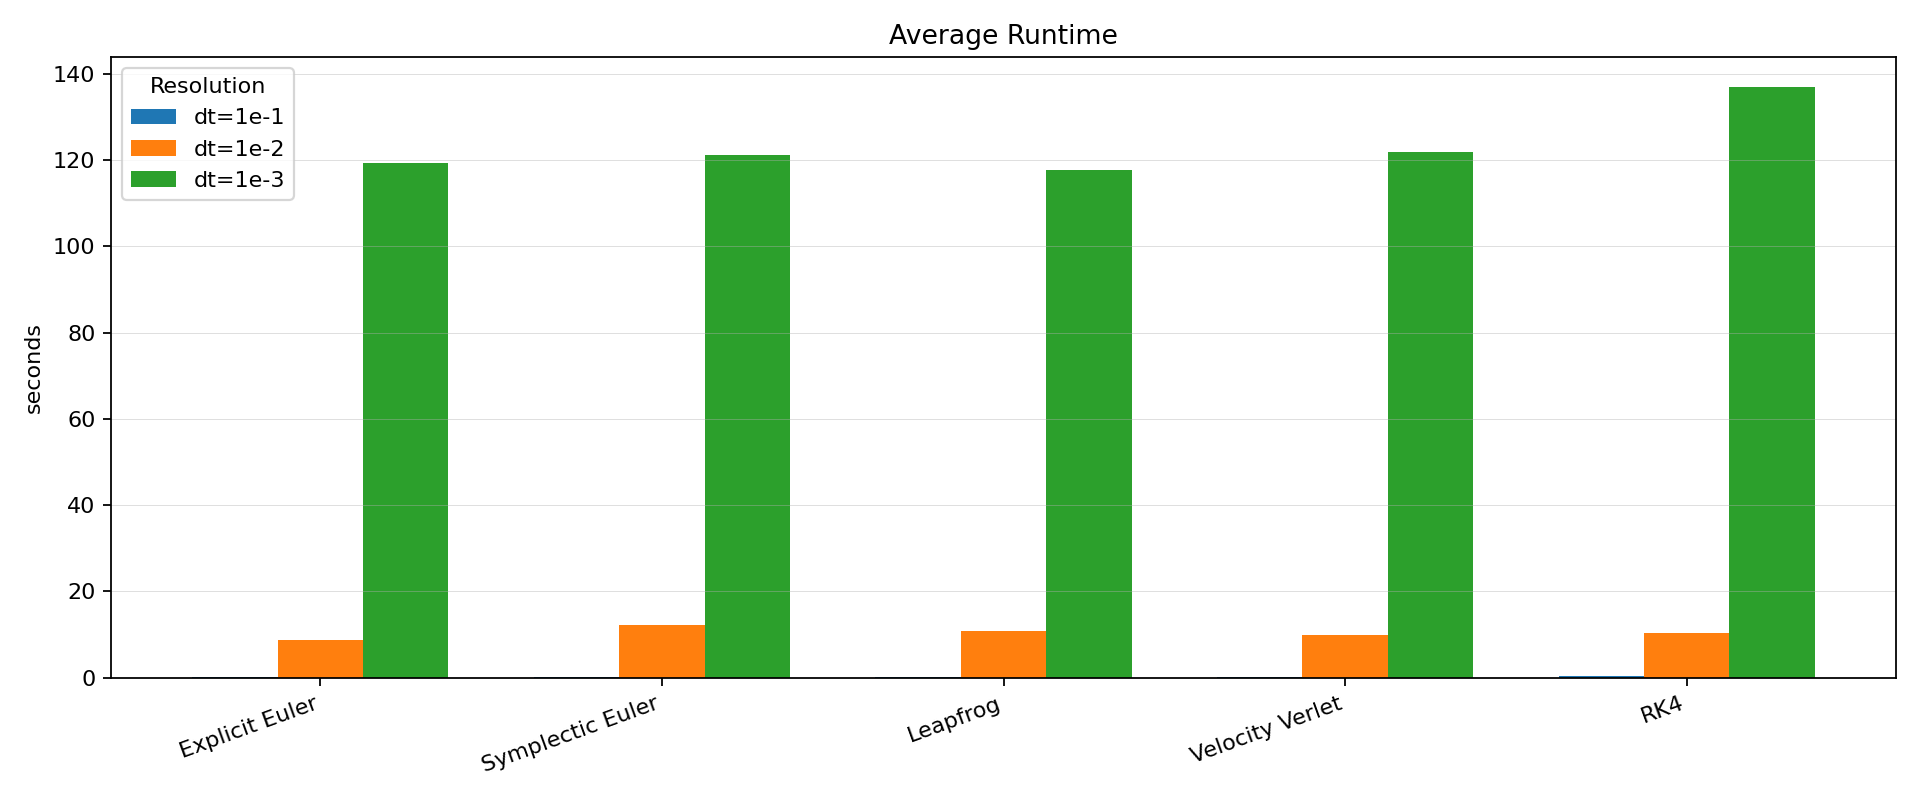
\includegraphics[width=1\textwidth]{figures/preliminary/average_runtime_seconds.png}
    \caption{Average Integrator Runtime}
\end{figure}

\subsection{Energy Conservation}

Figure 2 presents the distribution of relative energy errors for each integrator across the three tested
timesteps. Explicit Euler sits consistently around a relative error of $10^0$ regardless of resolution, with a
very narrow spread, indicating that the method fails to conserve energy irrespective of how finely the
timestep is refined. Symplectic Euler, Leapfrog, and Velocity Verlet all show a clear downward trend in
error as the timestep decreases, which is expected of lower-order methods whose local truncation error
scales with $\Delta t$. RK4 displays the widest spread of the five integrators, ranging from below $10^{-12}$
at $\Delta t = 10^{-3}$ up to over $10^1$ at $\Delta t = 10^{-1}$, showing that its performance is highly
sensitive to the choice of timestep.

\begin{figure}[h]
    \centering
    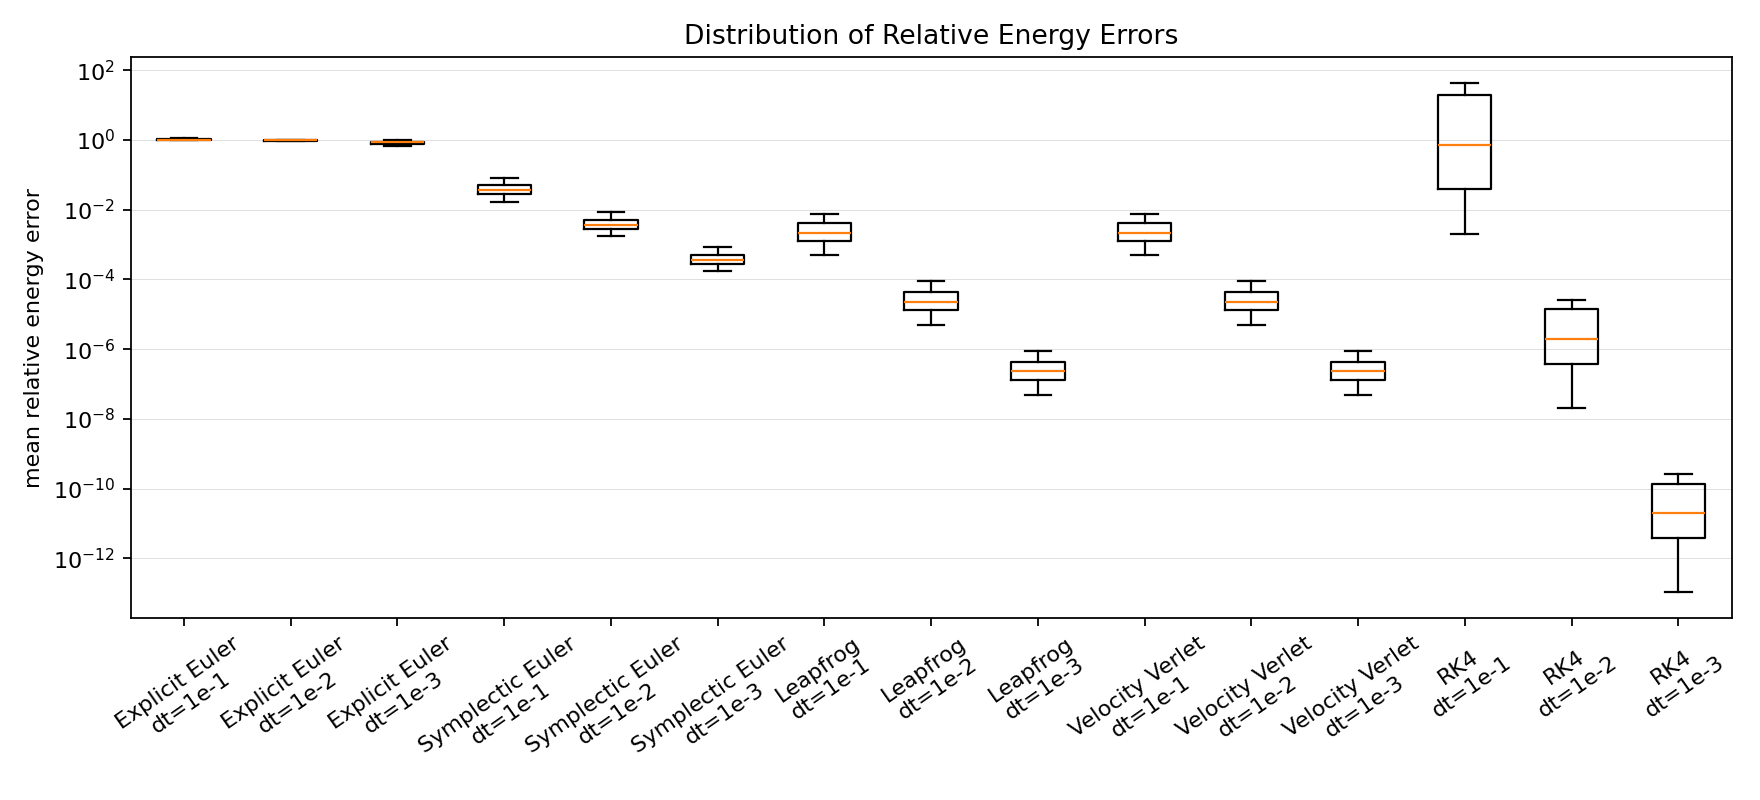
\includegraphics[width=1\textwidth]{figures/preliminary/energy_error_boxplot.png}
    \caption{Relative Energy Error Box Plot}
\end{figure}

Figure 3 shows the mean relative energy error plotted directly against timestep on a log-log scale. Explicit
Euler remains flat at approximately $10^0$ across all three timesteps, confirming the boxplot observation
that reducing $\Delta t$ does not meaningfully improve its energy behaviour over the tested range. Symplectic
Euler and Velocity Verlet both decrease steadily as the timestep shrinks, with Velocity Verlet consistently
outperforming Symplectic Euler by roughly two orders of magnitude at a given resolution. Leapfrog overlaps
almost exactly with Velocity Verlet on this plot, which is unsurprising given the two schemes are algebraically
equivalent formulations of the same method. RK4 is the standout here: at $\Delta t = 10^{-1}$ it produces the
worst energy error of all five integrators, exceeding even Explicit Euler, yet at $\Delta t = 10^{-3}$ it
produces the best energy error by several orders of magnitude, dropping below $10^{-8}$.

\begin{figure}[h]
    \centering
    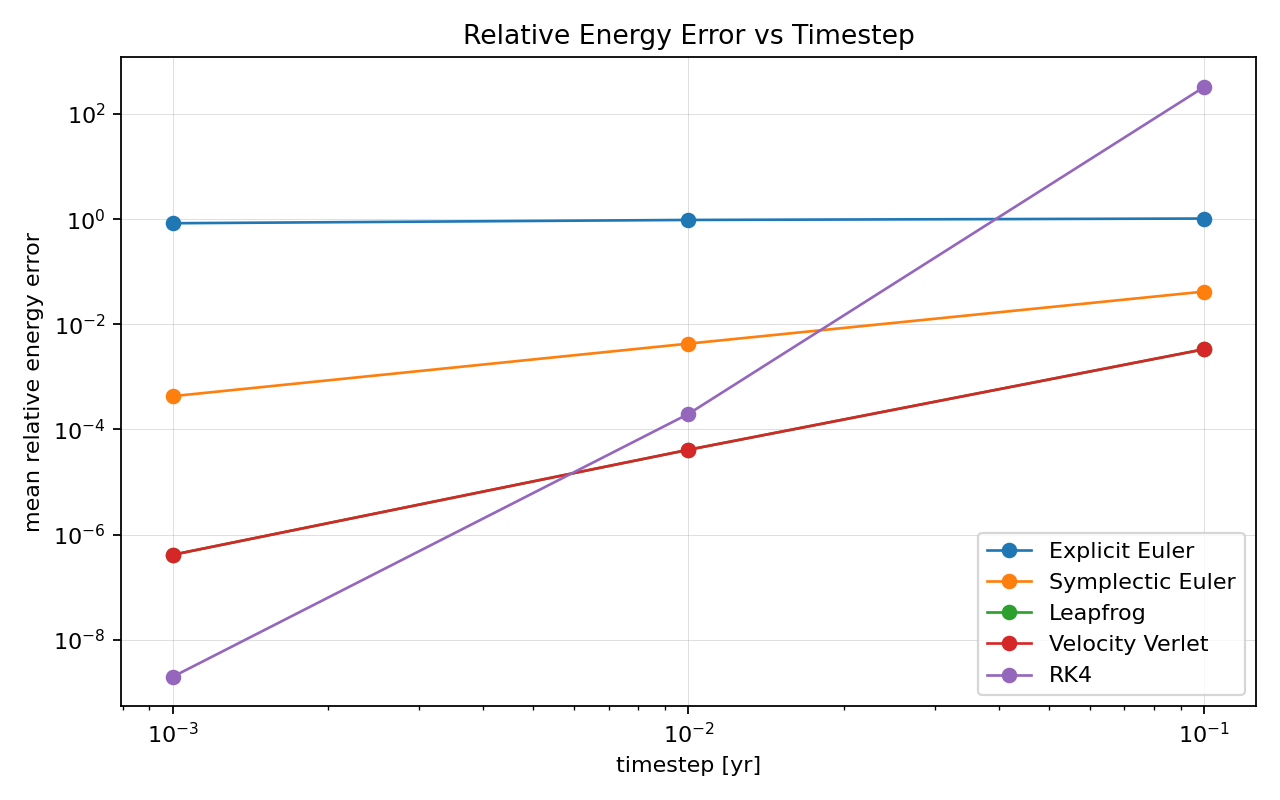
\includegraphics[width=1\textwidth]{figures/preliminary/energy_error_vs_timestep.png}
    \caption{Relative Energy Error vs Timestep}
\end{figure}

Figures 4 through 6 break the mean, median, and maximum relative energy error down by integrator and
resolution as grouped bar charts. All three present essentially the same ranking: at $\Delta t = 10^{-3}$,
the ordering from worst to best is Explicit Euler, Symplectic Euler, then Leapfrog and Velocity Verlet
together, with RK4 producing the smallest error of the group by a wide margin. The maximum relative
energy error (Figure 6) makes the instability of RK4 at coarse timesteps most visible, with a value on the
order of $10^4$ at $\Delta t = 10^{-1}$, several orders of magnitude above every other integrator at the
same resolution.

\begin{figure}[h]
    \centering
    
\includegraphics[width=1\textwidth]{figures/preliminary/mean_relative_energy_error.png}
    \caption{Mean Relative Energy Error by Integrator and Resolution}
\end{figure}

\begin{figure}[h]
    \centering
    
\includegraphics[width=1\textwidth]{figures/preliminary/median_relative_energy_error.png}
    \caption{Median Relative Energy Error by Integrator and Resolution}
\end{figure}

\begin{figure}[h]
    \centering
    
\includegraphics[width=1\textwidth]{figures/preliminary/max_relative_energy_error.png}
    \caption{Maximum Relative Energy Error by Integrator and Resolution}
\end{figure}

Finally, Figure 7 shows the mean absolute energy conservation value for each integrator. Explicit Euler,
Symplectic Euler, Leapfrog, and Velocity Verlet all sit near zero on this linear scale at every resolution
tested. RK4 is the only integrator to depart visibly from zero, and only at $\Delta t = 10^{-1}$, where the
mean energy value rises to approximately $0.029$, consistent with the instability already noted in Figures
3 and 6.

\begin{figure}[h]
    \centering
    
\includegraphics[width=1\textwidth]{figures/preliminary/mean_energy.png}
    \caption{Mean Energy Conservation by Integrator and Resolution}
\end{figure}

\subsection{Angular Momentum Conservation}

Figure 8 plots the mean relative angular momentum error against timestep for each integrator. Explicit
Euler again remains flat at approximately $10^0$ across the tested range, mirroring its behaviour for
energy conservation. Symplectic Euler, Leapfrog, and Velocity Verlet all sit near the floating-point noise
floor, around $10^{-13}$, and are largely insensitive to the choice of timestep, which is consistent with
the fact that these are symplectic integrators applied to a central force problem where angular momentum
is an exactly conserved quantity of the underlying Hamiltonian. RK4 again shows the steepest dependence on
timestep of any integrator, falling from just below $10^0$ at $\Delta t = 10^{-1}$ to below $10^{-9}$ at
$\Delta t = 10^{-3}$.

\begin{figure}[h]
    \centering
    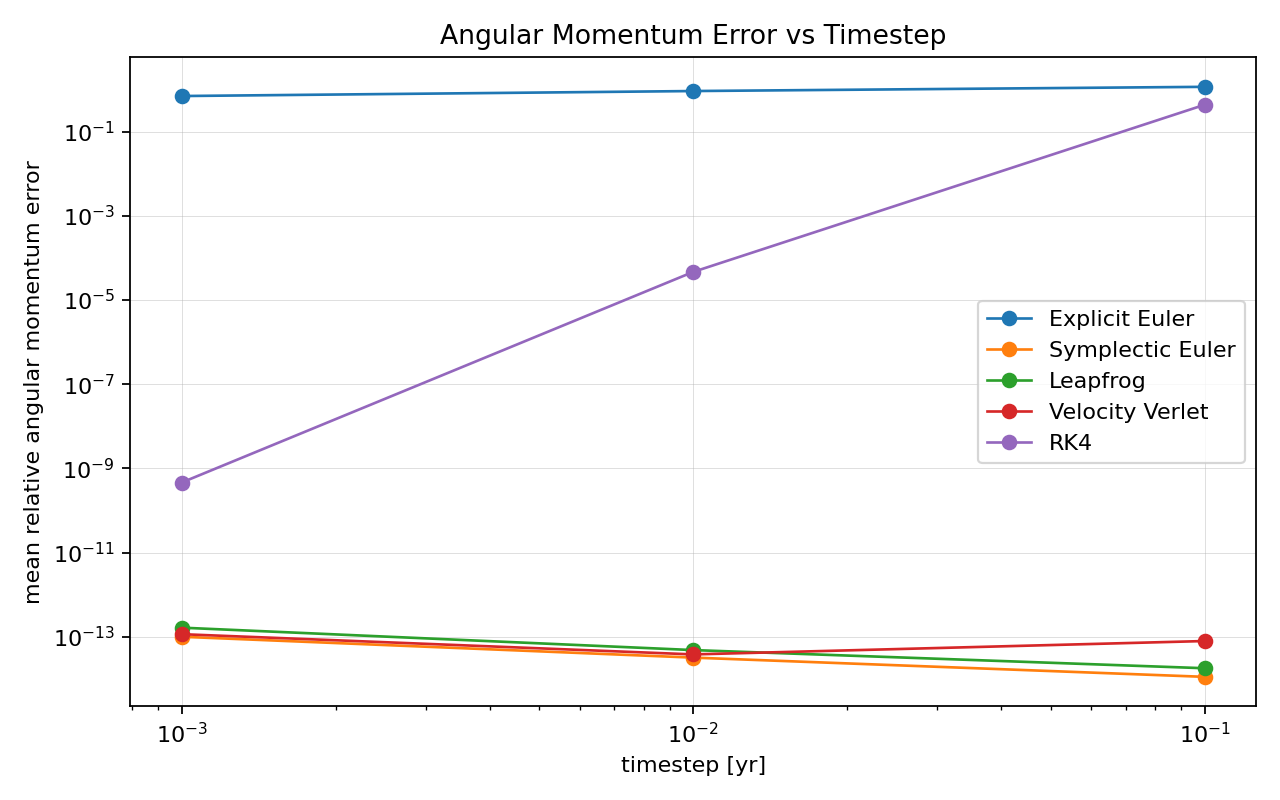
\includegraphics[width=1\textwidth]{figures/preliminary/angular_momentum_error_vs_timestep.png}
    \caption{Angular Momentum Error vs Timestep}
\end{figure}

Figures 9 through 11 present the mean, median, and maximum relative angular momentum error broken down
by integrator and resolution. Across all three, Symplectic Euler, Leapfrog, and Velocity Verlet remain
several orders of magnitude below Explicit Euler and RK4 at every resolution, with their error values
hovering around $10^{-13}$ regardless of timestep. RK4 is the only integrator among the five whose angular
momentum error responds strongly to a decrease in timestep, improving from around $10^{-1}$ at
$\Delta t = 10^{-1}$ to around $10^{-9}$ at $\Delta t = 10^{-3}$ in the mean case.

\begin{figure}[h]
    \centering
    
\includegraphics[width=1\textwidth]{figures/preliminary/mean_relative_angular_momentum_error.png}
    \caption{Mean Relative Angular Momentum Error by Integrator and Resolution}
\end{figure}

\begin{figure}[h]
    \centering
    
\includegraphics[width=1\textwidth]{figures/preliminary/median_relative_angular_momentum_error.png}
    \caption{Median Relative Angular Momentum Error by Integrator and Resolution}
\end{figure}

\begin{figure}[h]
    \centering
    
\includegraphics[width=1\textwidth]{figures/preliminary/max_relative_angular_momentum_error.png}
    \caption{Maximum Relative Angular Momentum Error by Integrator and Resolution}
\end{figure}

Figure 12 shows the mean absolute angular momentum value for each integrator. Symplectic Euler, Leapfrog,
and Velocity Verlet produce an identical value across all three resolutions, at approximately $7.7 \times
10^{-5}$, indicating exact conservation to within floating-point precision independent of timestep.
Explicit Euler departs from this value and drifts further as the timestep increases, while RK4 also departs
from the reference value, most noticeably at $\Delta t = 10^{-1}$.
 
\begin{figure}[h]
    \centering
    
\includegraphics[width=1\textwidth]{figures/preliminary/mean_angular_momentum.png}
    \caption{Mean Angular Momentum Conservation by Integrator and Resolution}
\end{figure}